\chapter{Thesis' Planning}
\label{chapter:planning}

The planned work to be continued after the end of \textit{Introduction to the Research in Electrical and Computer Engineering} is represented in Figure~\ref{fig:gantt}.

\begin{figure}[!htb]
	\centering
	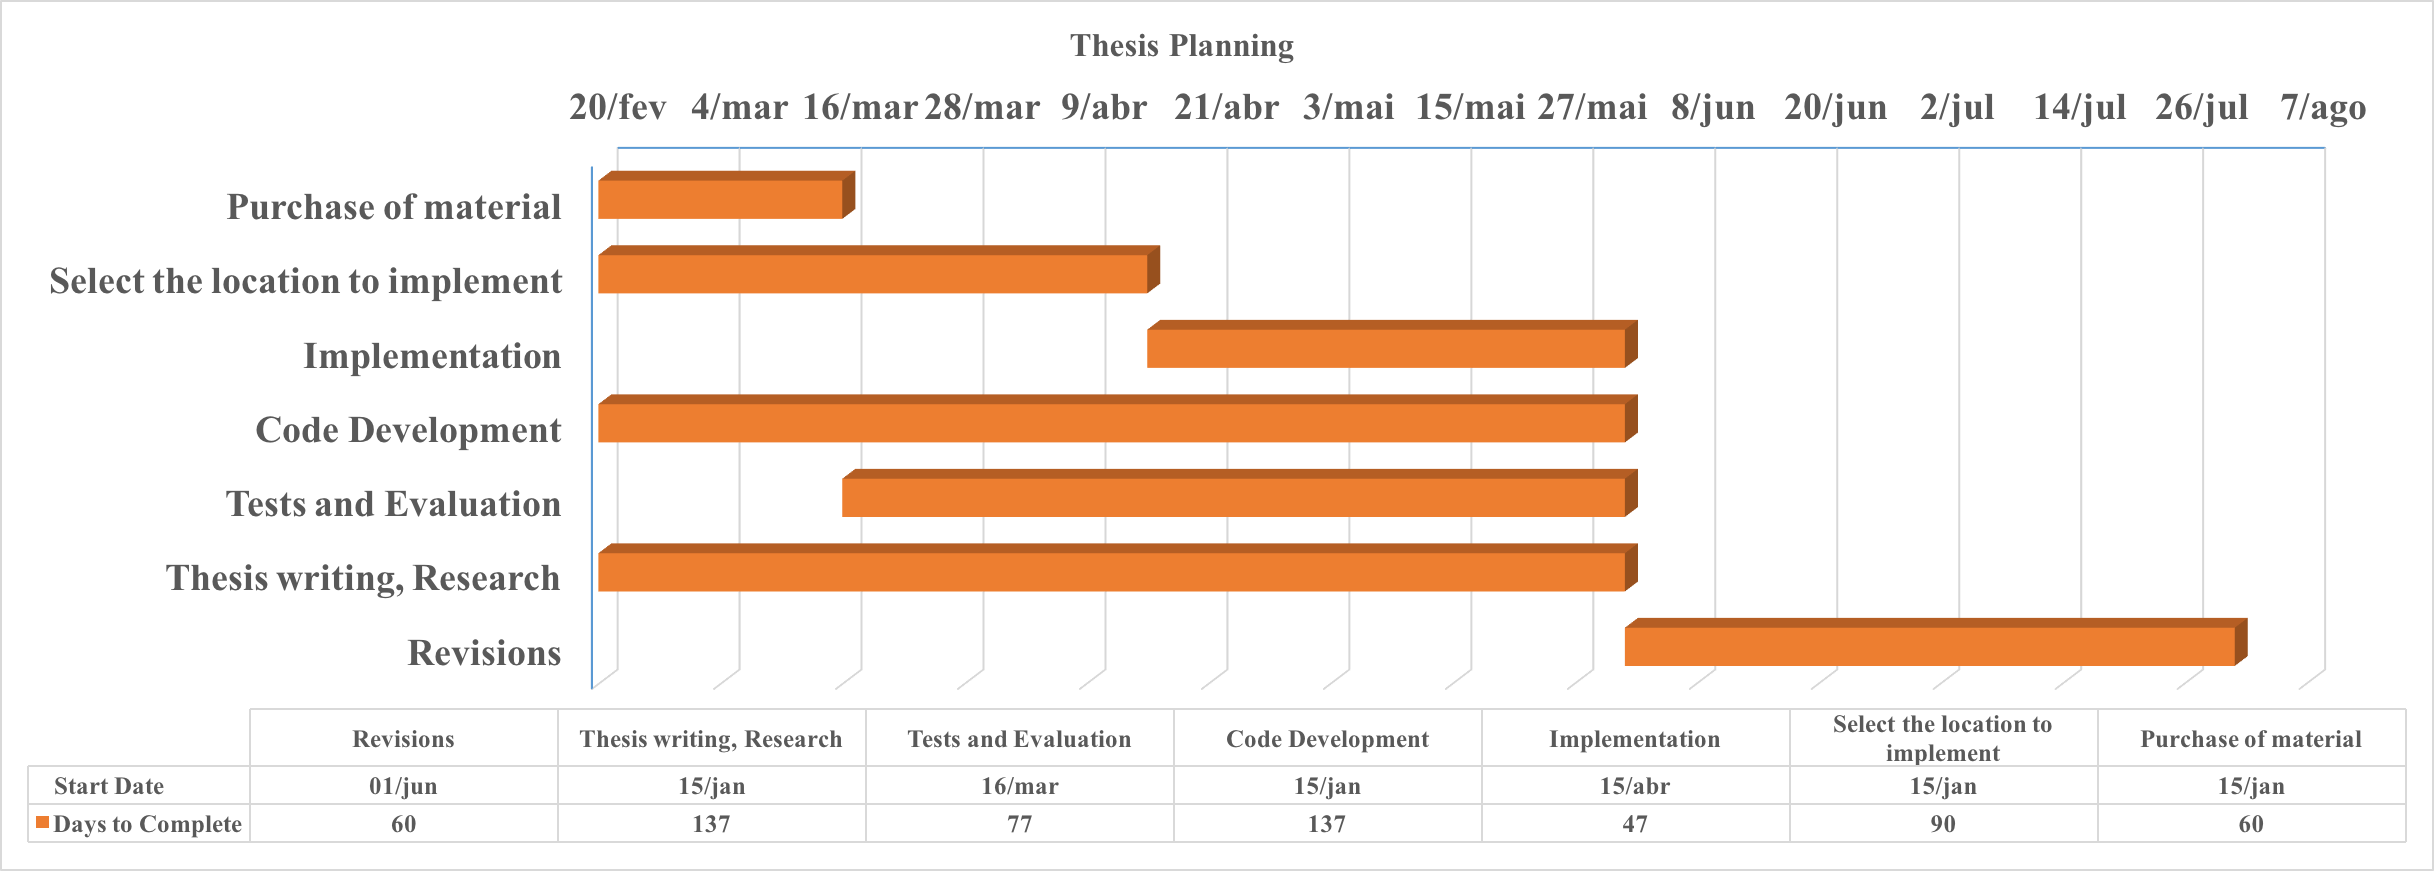
\includegraphics[width=1\textwidth]{Figures/gantt_v2.png}
	\caption[Gantt Diagram]{Gantt diagram.}
	\label{fig:gantt}
\end{figure}

Currently, we have already started the process of purchase of the necessary material, more specifically the Bluetooth beacons, and plan where to implement the positioning system. In addition to these two tasks, the code to perform the algorithm (Lateration~(\ref{subsection:lateration}) and/or Fingerprinting~(\ref{subsection:fingerprinting})) and the communication between the mobile phone application (\ref{section:app}) and the back-end (\ref{section:backend}) will be developed. After receiving the beacons, code related to these, such as beacon detection and acquirement of their \gls{rssi} and \gls{uuid} by the application, will be developed and tested in the first scenario nominative in Section~\ref{section:scenarios}.

As soon as the place to implement the system is chosen, the implementation starts in the second scenario indicated in~\ref{section:scenarios}, making at the same time, if needed, changes in the code or bug fixes.

The writing of the thesis will be carried out during the course of the tasks described previously. Implementation, Evaluation and Conclusion will be developed and finalized as the work progresses.

After the completion of these tasks, a review time is provided to make unexpected changes.

Delivery is estimated to be between June 1 and July 31. The discussion of the thesis must be performed after the delivery of the same, sometime no later than October.
